\documentclass[11pt, a4paper, spanish, openright, twoside]{book}
\usepackage[spanish, activeacute]{babel}
\usepackage[utf8]{inputenc}
%\usepackage[top=2.5cm, bottom=2.5cm, outer=1.75cm, inner=1.75cm, heightrounded, marginparwidth=2.5cm, marginparsep=0.3cm]{geometry}	%márgenes empequeñecidos
\usepackage[top=2.95cm, bottom=2.25cm, outer=2.75cm, inner=2.75cm, heightrounded, marginparwidth=2.5cm, marginparsep=0.3cm]{geometry}	%márgenes originalmente
\usepackage{dpg}
\usepackage{fli}

\usepackage{pgf}
\usepackage{tikz}

\usepackage[figuresright]{rotating}
\usepackage{graphicx}
\usepackage{wrapfig}
\usepackage{lscape}
\usepackage{rotating}
\usepackage{epstopdf}

\usepgflibrary{shapes.geometric} % LATEX and plain TEX and pure pgf
\usetikzlibrary{arrows,automata,positioning}
\tikzstyle{accepting by double}= [double distance=1.6pt,double,outer sep=.5\pgflinewidth+.8pt] % esto es algo estético.
\renewcommand\shorthandsspanish{}  % para compatibilizar spanish con tikz

%%%%%%		Figuras		%%%%%%%%%%%%%%%%%%%
\usepackage[vflt]{floatflt}		%Entorno float-figure

%%%%%%		Page style		%%%%%%%%%%%%%%%%%%%
\renewcommand{\thepage}{\arabic{page}}% Arabic page numbers\fancyhead{}
\pagestyle{fancy}
\fancyfoot{}
\fancyhead[LO,RE]{Práctica 11}	%encabezado de pares: nombre de la sección
\fancyhead[RO,LE]{Aprendizaje automático con WEKA}
\fancyfoot[LE,RO]{\thepage}	%abajo a izqda en pares, derecha en impares: numero de pagina
%\fancyhead[LE]{\nouppercase{\leftmark}} %cuadro izquierdo de pagina par: parte y contador
\fancyfoot[CE]{Inteligencia Artificial} 
\fancyfoot[CO]{Doble Grado Informática-Matemáticas - Universidad Complutense}
\renewcommand{\footrulewidth}{0.4pt}
\renewcommand{\headrulewidth}{0.4pt}		% linea por debajo del encabezado
\renewcommand{\sectionmark}[1]{\markright{\textbf{\thesection. #1}}}	%negrita
\renewcommand{\labelitemi}{$\circ$} %Primer itemize con circunferencia vacia
\renewcommand{\labelitemii}{$\cdot$} %Segundo itemize con punto pequeño \cdot
\renewcommand*{\thesection}{\arabic{section}}	% Hace que no apareca el indice de capitulos y que comience en section

%%%%%%		Others		%%%%%%%%%%%%%%%%%%%
\setlength{\leftmarginii}{0em} %Segundo itemize sin sangria
\setlength{\leftmarginiii}{1em} %Tercer itemize casi sin sangria
\renewcommand{\labelitemiii}{ }
\pagenumbering{roman}
\addto{\captionsspanish}{\renewcommand*{\contentsname}{Índice}} %Cambia "Indice general" por "Indice"



\begin{document} 
\title{\Huge{\textsc{Inteligencia Artificial}} \\
	\vspace{0.7cm}
	 \textsc{\Large{Práctica 11}} \\
	\vspace{1.5cm}
	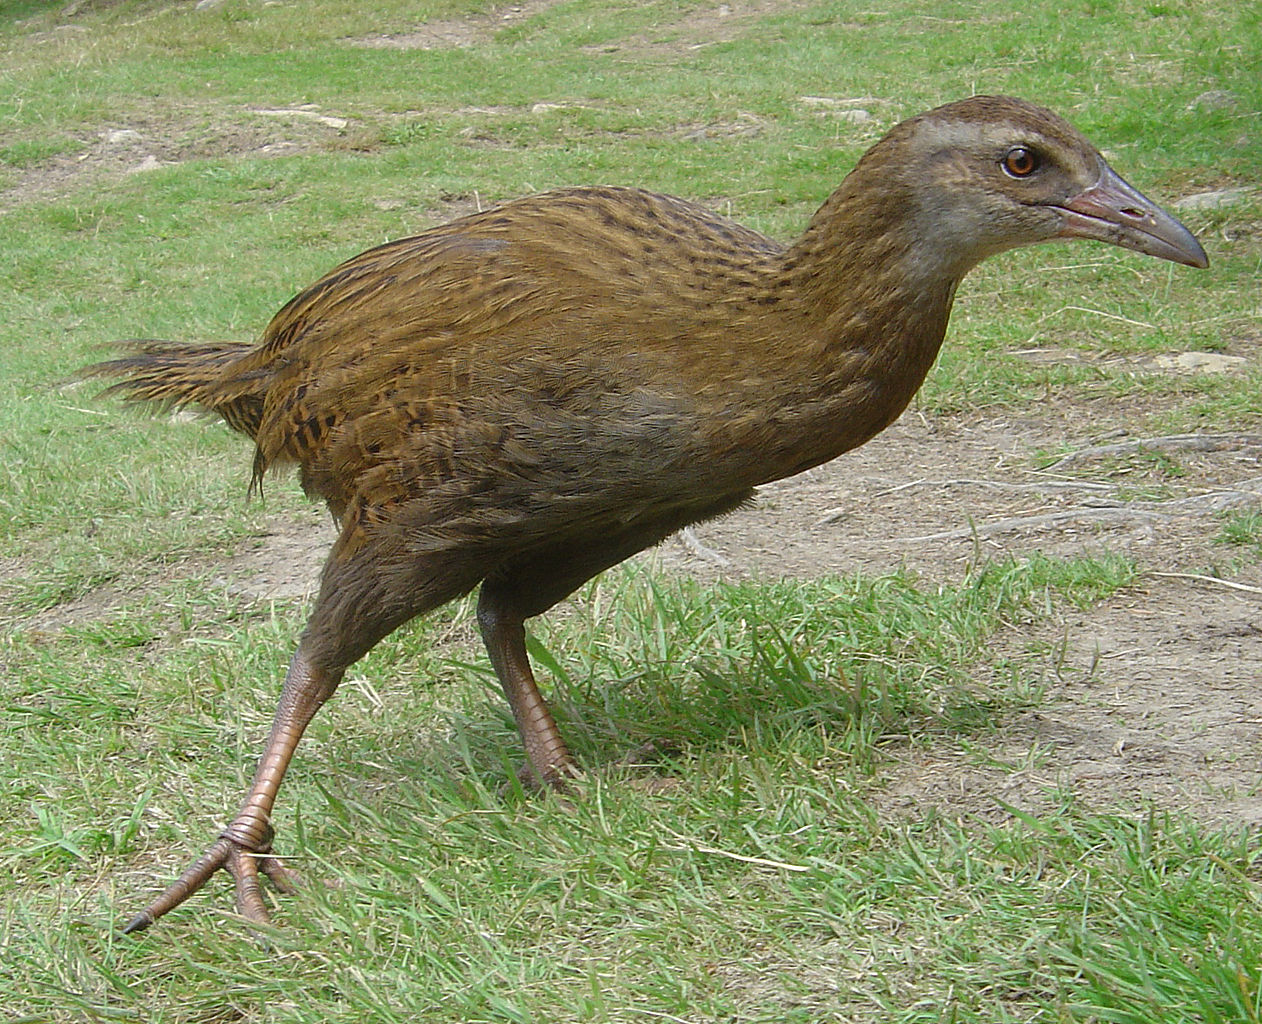
\includegraphics[scale=0.2]{weka}
	}
\author{\textsc{Grupo 3:}\\
	Enrique Ballesteros Horcajo\\
	Ignacio Iker Prado Rujas}
\date{\Today}
\maketitle

\newpage
\mbox{}
\thispagestyle{empty}						% Hoja en blanco, sin numeros ni nada
\newpage


\tableofcontents 							%INDICE hipervinculado

\newpage
\mbox{}
\thispagestyle{empty}						% Hoja en blanco, sin numeros ni nada
\newpage

\pagenumbering{arabic}						% Pone el contador de paginas a 1 y ahora en numeros normales

\vspace{3cm}


\newpage

\begin{section}*{Introducción}
	
	En esta práctica vamos a trabajar con el entorno que nos proporciona WEKA\footnote{Página web de WEKA \href{http://www.cs.waikato.ac.nz/ml/weka/}{aquí}.}, aplicando herramientas de aprendizaje automático a conjuntos de datos dados por los ficheros \texttt{diabetes.arff} y \texttt{glass.arff}.
	
\end{section}

\begin{section}{Apartado 1}
	
	Durante todo este apartado los datos han sido tomados de \texttt{diabetes.arff} incluido en el subdirectorio data de la distribución de WEKA, en el campus virtual. Este dataset contiene los resultados de un estudio relacionado con la diabetes.
	
	\begin{itemize} 
	\item \textit{Analiza el archivo citado y contesta las siguientes preguntas: ¿Cuántas instancias hay? ¿Cuántos 
	atributos se utilizan? ¿Por qué atributo queremos aprender a clasificar?}

	Hay 768 instancias. Se utilizan nueve atributos, ocho como datos (edad, peso, etc.)  y uno para clasificar (ser o no diabético). Queremos aprender a clasificar por este último.
 
	\item \textit{Ejecuta J48 (versión WEKA de C4.5). Utiliza para la validación el “training set”. Incluye en la 
	memoria los resultados obtenidos y la representación gráfica del árbol correspondiente.}


\begin{sidewaysfigure}
	\hspace{-1cm}
	\scalebox{0.74}{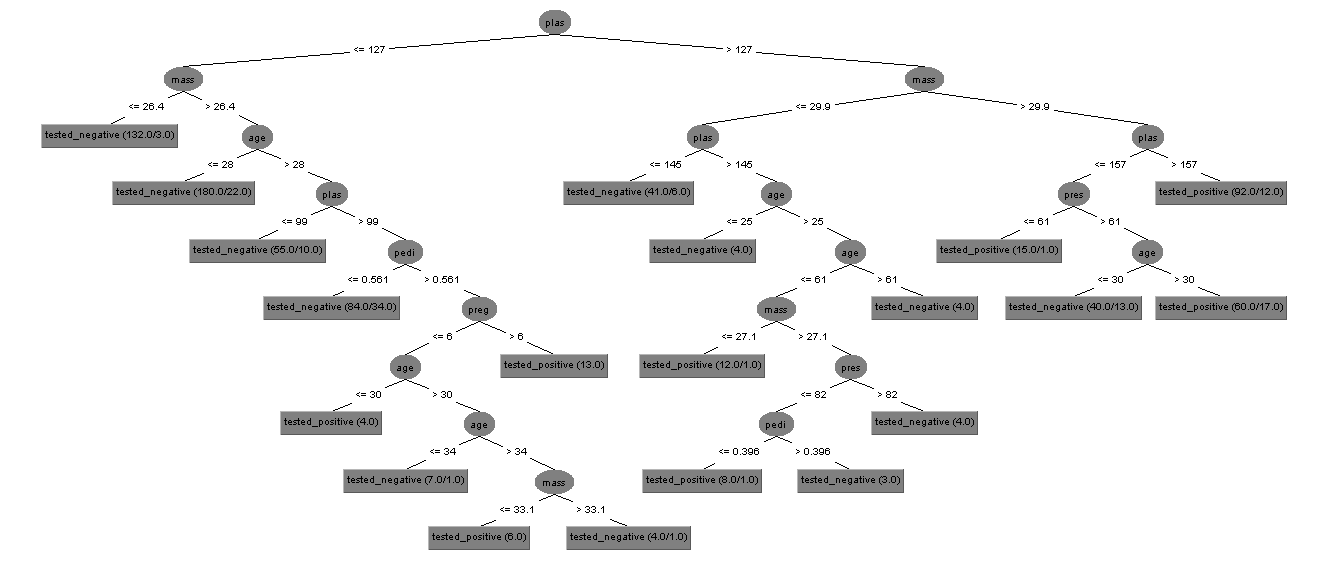
\includegraphics{arbol}}
    	\caption{Gráfica del árbol correspondiente a los resultados de la ejecución de J48, con validación “training set”.}
\end{sidewaysfigure}

\noindent\fbox{
    \parbox{\textwidth}{

\begin{center}=== Classifier model (full training set) ===	

\vspace{0.2cm}
\textit{(El ábol se muestra en una figura a parte, en la página siguiente)}
\vspace{0.2cm}

Number of Leaves  : 	20

Size of the tree : 	39 \\

\vspace{0.2cm}
	=== Evaluation on training set === \\
	=== Summary ===

 \begin{tabular}{ll}
Correctly Classified Instances    &     646         \quad      84.1146 \% \\
Incorrectly Classified Instances   &    122        \quad       15.8854 \% \\
Kappa statistic                  &         \quad 0.6319 \\
Mean absolute error         &          \quad    0.2383 \\
Root mean squared error  &        \quad        0.3452 \\
Relative absolute error      &         \quad   52.4339 \% \\
Root relative squared error &       \quad      72.4207 \% \\
Total Number of Instances    &     \quad      768     
\end{tabular}

\vspace{0.2cm}
=== Detailed Accuracy By Class ===

\begin{flushright} 
\begin{tabular}{ccccccc}
                TP Rate  & FP Rate &  Precision &  Recall &  F-Measure &  ROC Area & Class \\
 		 0.936   &  0.336    &  0.839   &  0.936  &   0.885   &   0.888 &   tested\_negative \\
                 0.664    & 0.064     & 0.848   &  0.664   &  0.745    &  0.888   &  tested\_positive \\
\hspace{-2.25cm}Weight. Avg.   0.841  &   0.241 &     0.842 &    0.841   &  0.836  &    0.888
\end{tabular}
\end{flushright}

\vspace{0.3cm}
=== Confusion Matrix ===

   a   b   $<$-- classified as \\
 468  32 $\mid$   a = tested\_negative \\
  90 178 $\mid$   b = tested\_positive \end{center}

}}

		\begin{itemize}
			 \item \textit{¿Cuántas instancias han sido mal clasificadas?}  
			
			Han sido mal clasificadas 122 instancias.
			
			\item \textit{¿Cuántos nodos terminales hay en el árbol?} 
			
			Hay 20 nodos terminales en el árbol.
			
			\item \textit{¿Por qué atributo se clasifica en el primer nivel del árbol?} 
			
			Se clasifica por plass (plasma glucose concentration a 2 hours in an oral glucose tolerance test).
			
		\end{itemize}

	\item  \textit{Vuelve a ejecutar J48 primero con ``cross-validation'' y después con ``percentage split'' (con un valor 
	del 66\%) y observa las diferencias. Haz una tabla con el porcentaje de instancias bien clasificadas en 
	cada uno de los tres métodos de validación. Incluye en esa tabla la precisión y el recall para cada 
	uno de los tres métodos.}

		\begin{center}
 			 \begin{tabular}{| c | c | c | c |}
 			   \hline
			     				       	  & Training set 	& Cross-validation 		& Percentage split  \\ \hline
			    Porcentaje bien clasificadas  	  & 84.1146 \% 	& 73.8281 \%		& 76.2452 \% \\ \hline			 
			    Recall 			     	  & 0.841  		& 0.738 			& 0.762 \\ \hline 
			    Precisión			      	  & 0.842  		& 0.735 			& 0.756  \\ \hline \hline
			    Precisión con negativos		  & 0.839		& 0.790			& 0.809 \\ \hline
			    Precisión con positivos 		  & 0.848 		& 0.632			& 0.644 \\ 
			    \hline
			  \end{tabular}
		\end{center}

		\begin{itemize}
			 \item \textit{Comenta los resultados obtenidos. }
			
			El porcentaje de bien clasificados es mejor en el primer método, sin embargo hay que explicar por qué es así. El training set crea la clasificación a partir de todos los ejemplos de entrenamiento  y luego la prueba sobre 
			los mismos ejemplos, por tanto siempre será el mejor método si se aplica sobre esos ejemplos de entrenamiento. Por ello nos fijaremos en los otros dos. El percentage split obtiene mejor porcentaje de clasificados, 
			y también mejor precisión tanto con negativos como con positivos. Los negativos son más fiables que los positivos, por lo que los positivos deberían ir acompañados de una prueba médica que confirme los resultados.
			
			\item  \textit{¿Cuál de las tres validaciones te parece más fiable? ¿Por qué?} 
			
			La cross-validation es más fiable, por lo que un 73\% puede ser un porcentaje de acierto cercano a la realidad. Esto se debe a que la cross-vallidation obtiene 
			unos resultados más uniformes que no dependen del orden en que se escojan los ejemplos de entrenamiento, sino que presenta una media entre diez percentage splits. Por tanto es más fiable.
			
			 \item \textit{¿Cuántos falsos negativos (FN) y falsos positivos (FP) se han obtenido con el “percentage split”?} 
			
			Con percentage split se obtienen 26 falsos negativos y 36 falsos positivos.
			
		\end{itemize}
	

	\end{itemize}
\end{section}

\begin{section}{Apartado 2}
	Para este apartado se utilizará el dataset contenido en el archivo \texttt{glass.arff} incluido en el subdirectorio
	data de la distribución de WEKA y en el campus virtual. Este dataset contiene datos sobre tipos de
	cristal según sus características.

	\begin{itemize}
	\item \textit{Analiza el dataset. ¿En cuántas clases se clasifican los ejemplares? ¿Cuántos atributos se utilizan?}

	En 7 clases distintas: building windows float processed, building windows non float processed, vehicle windows float  processed,  vehicle windows non float processed, containers, tableware y headlamps.
	Utilizan 9 atributos : RI (refractive index),  Na (Sodium), Mg (Magnesium),  Al (Aluminum), Si (Silicon),  K (Potassium), Ca (Calcium), Ba (Barium) y Fe (Iron). En función de las cantidades para cada cristal se clasificará cada 
	cristal en un tipo de los 7.

	\item \textit{Aplica el clustering jerárquico a este conjunto de datos para 7 clusters y comenta los resultados 
	obtenidos. ¿Qué clases han quedado mejor clasificadas?}
	
	Ninguna realmente. Puede decirse que el build wind float y el vehicle wind float son las mejor clasificadas, ya que al menos ha metido todos en el mismo cluster. O también, se puede decir que 
	el build wind non-float porque está en el cluster que lleva su nombre. Realmente es una clasificación que creemos no tiene mucha utilidad, pues mete todos en prácticamente la misma clase. 
	Es uno de los problemas que suelen presentarse en  el aprendizaje automático.
	
	\item \textit{Discretiza los atributos utilizando un filtro supervisado. ¿Qué horquillas se han generado para los 
	valores del Calcio? Vuelve a ejecutar el clustering jerárquico y compara los resultados con los 
	anteriores. ¿Qué clases han quedado mejor clasificadas?}

	Cuatro horquillas: De $-\infty$ a 7.02, de 7.02 a 8.315, de 8.315 a 10.075 y de 10.075 a $\infty$.

	Los headlamps han quedado mucho mejor clasificados, pues ahora la mayoría están en una clase propia. Los build wind non-float tienen uno más en ``su clase".

	En el resto no hay un cambio significativo.

	\item \textit{Con los atributos en su estado original, utiliza el algoritmo de clustering EM (Expectation 
	Maximization) y compara con los resultados anteriores.}
	
	Ha mejorado la clasificación de los containers, agrupándolos en una sola clase, pero ha empeorado la clasificación del resto dividiéndolos en distintos clusters.

	\begin{itemize}
	\item \textit{¿Qué clases han quedado mejor clasificadas?}
	
	Realmente ninguna, los containers los agrupa juntos, pero mete otros tipos de cristales en esa misma clase por lo que tampoco es una clasificación del todo buena.

	\item \textit{¿Qué método de los tres anteriores te parece más útil para este ejemplo? ¿Por qué? }

	El segundo puede ser mejor porque al menos te separa los headlamps y el resto. Sin embargo, ningún método acaba de resultar útil para el ejemplo porque 
	no clasifica bien los tipos de cristales al no ser capaz de distinguir entre ellos y meterlos en la misma clase.

	\item \textit{¿Podríamos haber utilizado un algoritmo de clasificación como J48? }

	Para clasificar por Type desde luego,  por ejemplo utilizando el 66\% de entrenamiento. Aunque clasifica correctamente solo la mitad de los cristales restantes.

	\item \textit{¿Qué habríamos obtenido con los algoritmos de clustering si no tuviéramos el atributo de clase?}

	Agrupa (casi) todos en una misma clase pues no es capaz de encontrar diferencias sutiles entre los distintos cristales que se dan, y de las que se obtienen las diferentes clasificaciones. 
	No es un problema de relajar las exigencias para cada clase, sino que no sabe qué exigir para poder distinguir unas de otras.

	 \item \textit{¿En qué casos sólo podríamos utilizar clustering?}
	
	Si no tuviésemos las distintas clasificaciones por tipo de cristal, sin ejemplos de entrenamiento, solo podríamos utilizar el clustering para agrupar los cristales en clases diferentes.
	\end{itemize}
	\end{itemize}
\end{section}

	
\begin{thebibliography}{9}

\bibitem{aima}
	Russell, S.; Norvig, P, \\
	\emph{Artificial Intelligence, a modern aproach}.\\
	New Jersey: Pearson, 2010.
	
\bibitem{clase}
	Apuntes y transparencias de Inteligencia Artificial, \\
	Doble Grado Matemáticas - Ing. Informática, U.C.M., 2014-2015.

\end{thebibliography}


\end{document}